\documentclass[aspectratio=169]{beamer}

\usetheme{CERN}

\beamertemplatenavigationsymbolsempty

\usepackage{graphicx}
\usepackage{booktabs}

\usepackage{xcolor}
\usepackage{graphicx}
\usepackage{multicol}
\usepackage{wrapfig}

\graphicspath{ {images/} }
\usepackage[export]{adjustbox}

%----------------------------------------------------------------------------------------
%	TITLE PAGE
%----------------------------------------------------------------------------------------

\title[Configuration Management @ CERN]{Configuration Management @ CERN\\*Going Agile with Style}
\author{Andrea Giardini}
\date{\today}

\institute[CERN]
{
CERN \\
\medskip
\textit{andrea.giardini@cern.ch}
}
\date{24 April 2015 - PuppetCamp Berlin} % Date, can be changed to a custom date


\begin{document}

\cernSplashBlue

\begin{frame}
\titlepage
\end{frame}

\begin{frame}
\frametitle{Overview}
\tableofcontents
\end{frame}

%----------------------------------------------------------------------------------------
%	PRESENTATION SLIDES
%----------------------------------------------------------------------------------------

%------------------------------------------------
\section{Introduction}
%------------------------------------------------

\subsection{What we do at CERN}

\begin{frame}

    \frametitle{What is CERN}
    \begin{minipage}[t]{0.95\textwidth}
        \begin{columns}
            \begin{column}{0.5\textwidth}
                \begin{itemize}
                    \item European Organization for Nuclear Research
                    \item Situated in the border between Switzerland and France
                    \item 21 Member states
                    \item Big challenges 
                \end{itemize}
            \end{column}
            \begin{column}{0.5\textwidth}
                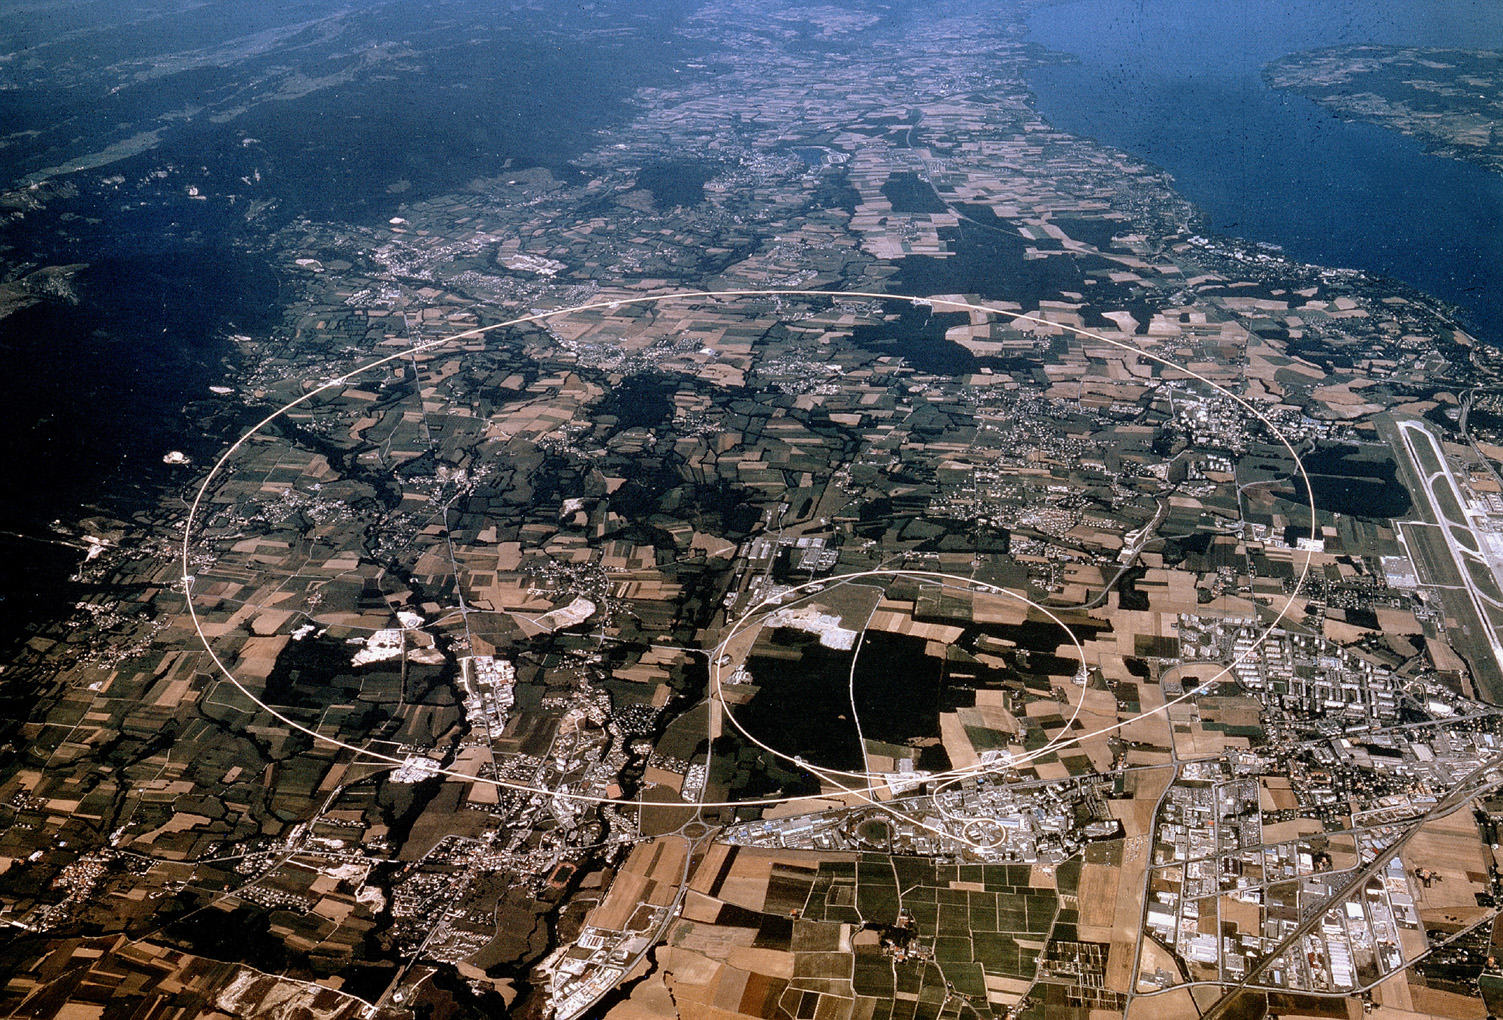
\includegraphics[width=1.1\textwidth]{CernMap.jpg}
            \end{column}
        \end{columns}
    \end{minipage}

\end{frame}

%------------------------------------------------

\begin{frame}
    \frametitle{Big Challenges - The FCC}
    \begin{center}
    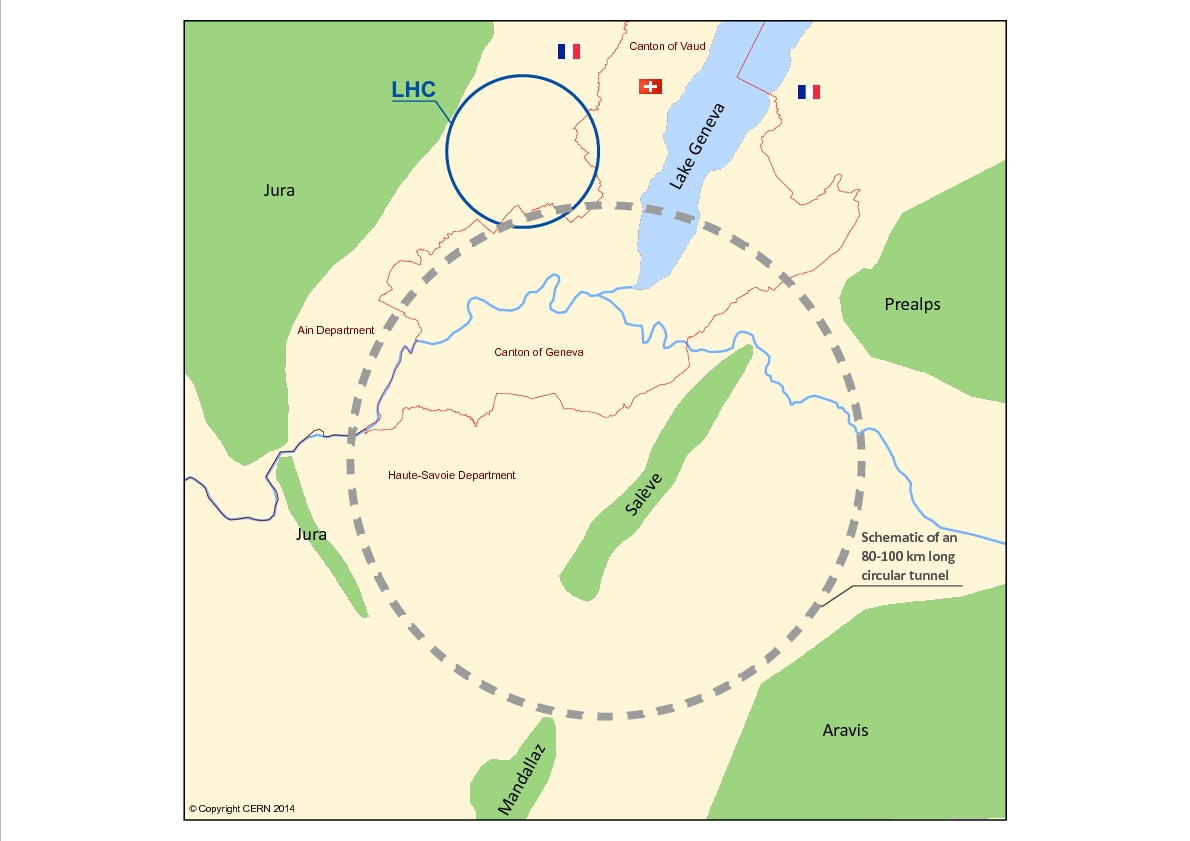
\includegraphics[width=0.65\textwidth,trim=4 4 4 4,clip]{CERN_LCC.jpg}
\end{center}
\end{frame}

%------------------------------------------------

\begin{frame}
    \frametitle{The LHC}
    \begin{center}
    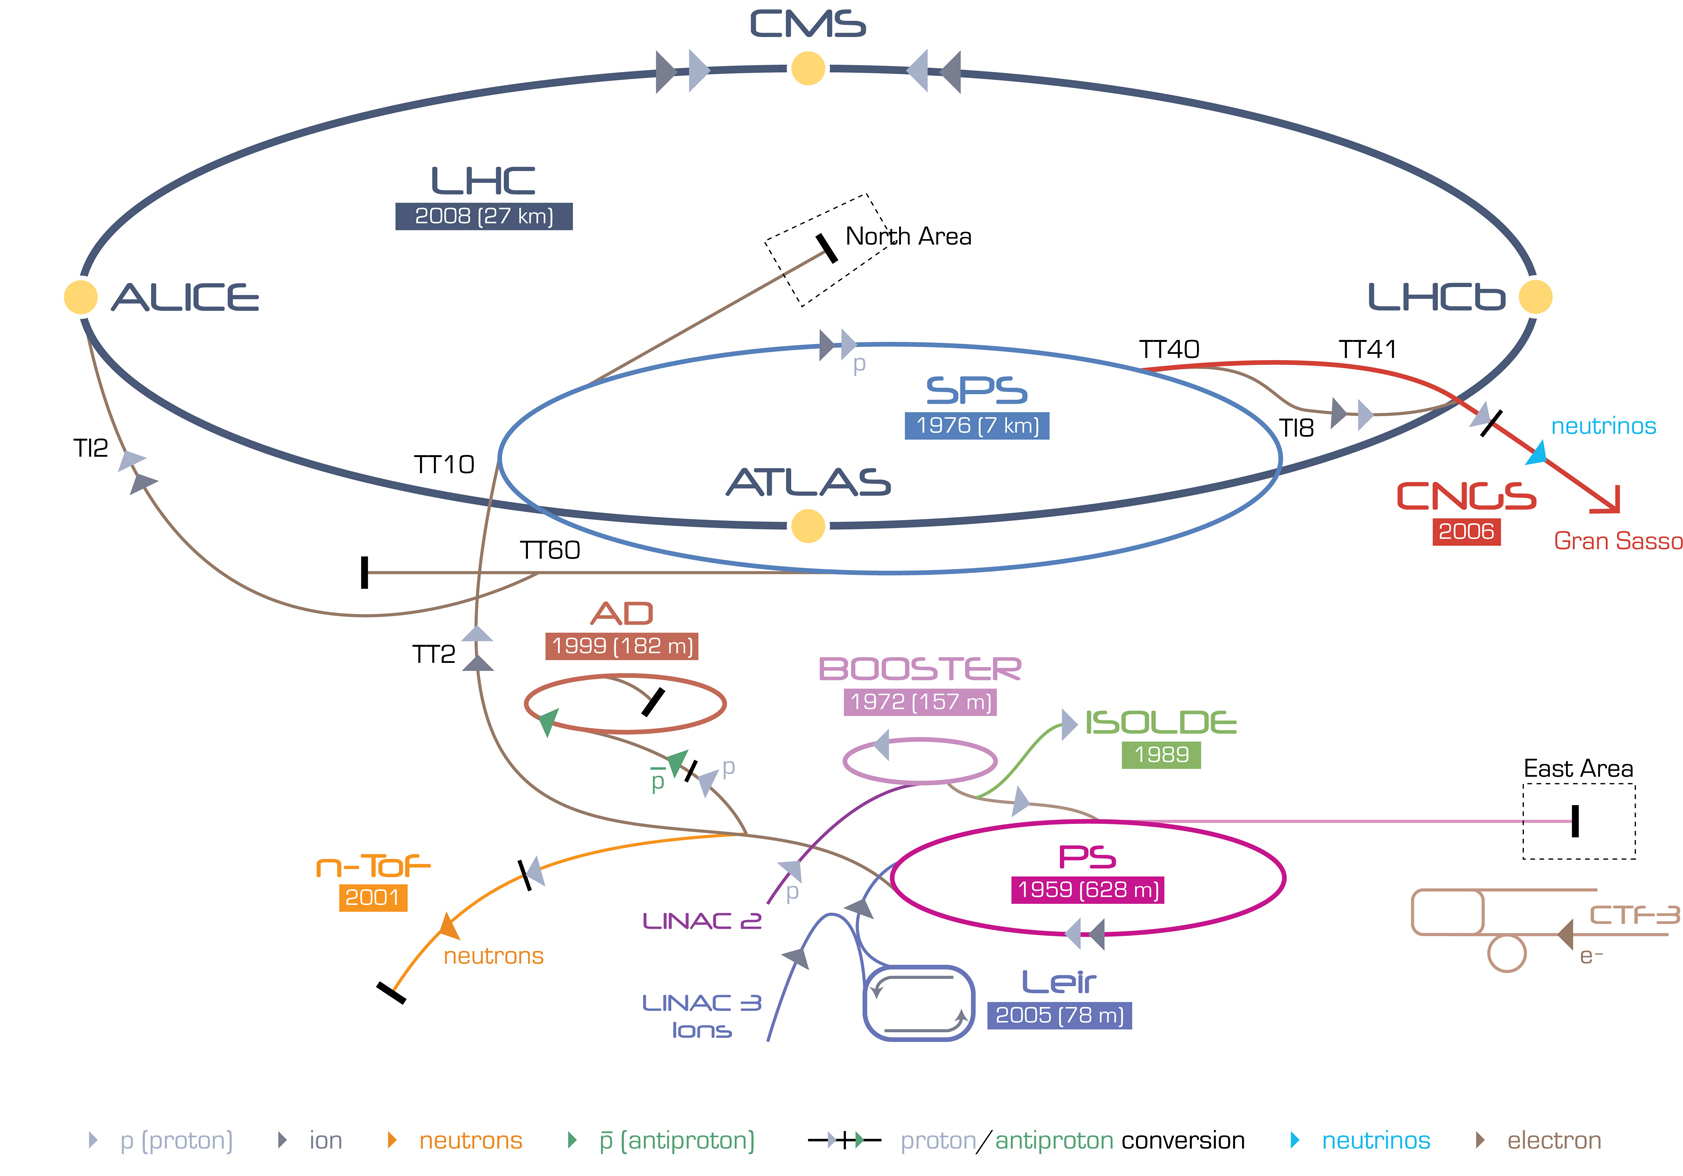
\includegraphics[width=0.65\textwidth,trim=4 4 4 4,clip]{Cern-Accelerator-Complex2.jpg}
\end{center}
\end{frame}

%------------------------------------------------

\begin{frame}
    \frametitle{The Accelerators}
    \begin{center}
    \includegraphics[width=0.7\textwidth,trim=4 4 4 4,clip]{Atlas.jpg}
    \end{center}
\end{frame}

%------------------------------------------------

\begin{frame}
    \frametitle{Data Flow}
    \begin{center}
    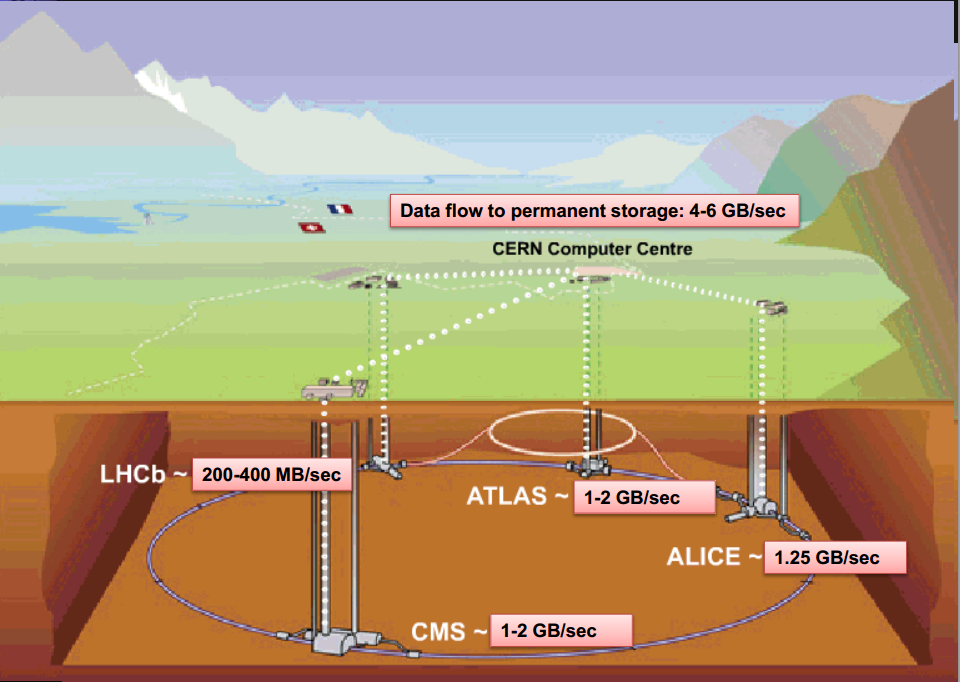
\includegraphics[width=0.65\textwidth,trim=4 4 4 4,clip]{LHC_DataFlow.png}
    \end{center}
\end{frame}

%------------------------------------------------

\subsection{Datacenters in Numbers}
\begin{frame}
    \frametitle{Datacenters}
    \begin{minipage}[t]{0.95\textwidth}
        \begin{columns}[T]
            \begin{column}{0.5\textwidth}
                Two datacenters:
                \begin{itemize}
                    \item Budapest
                    \item Geneva
                \end{itemize}
                Two dedicated links:
                \begin{itemize}
                    \item 2 x 100Gbps
                \end{itemize}
                \vspace{0.1in} 
                The number of resources is growing year by year.
                As today:
                \begin{itemize}
                    \item 15k servers
                    \item 100PB on tape
                    \item 200PB on disk
                \end{itemize}
            \end{column}
            \begin{column}{0.5\textwidth}
                \vspace{0.2in} 
                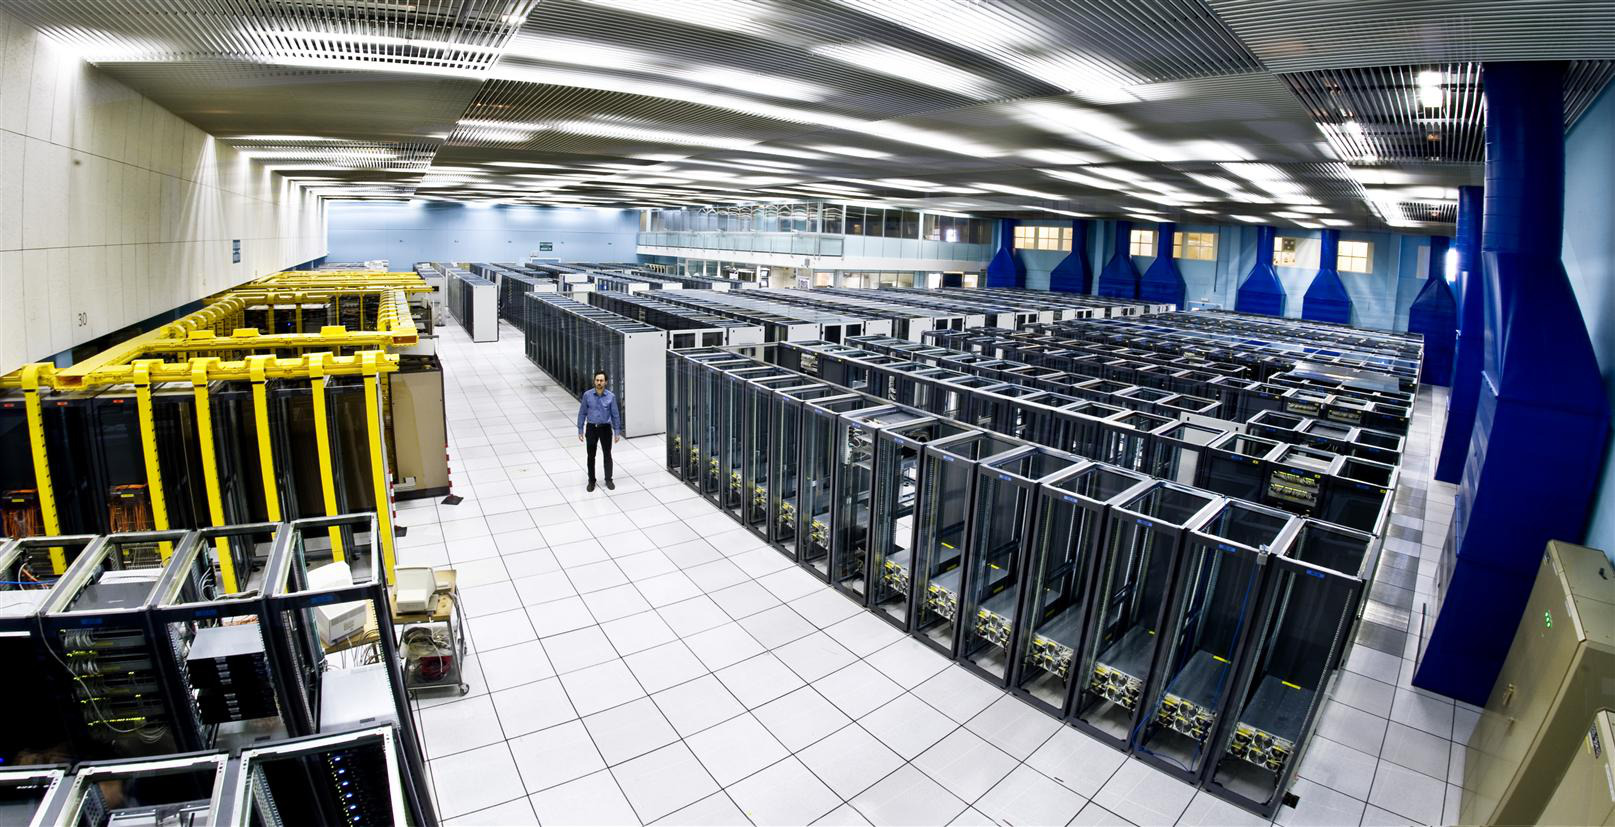
\includegraphics[width=1.1\textwidth]{DC_overview.png}
                %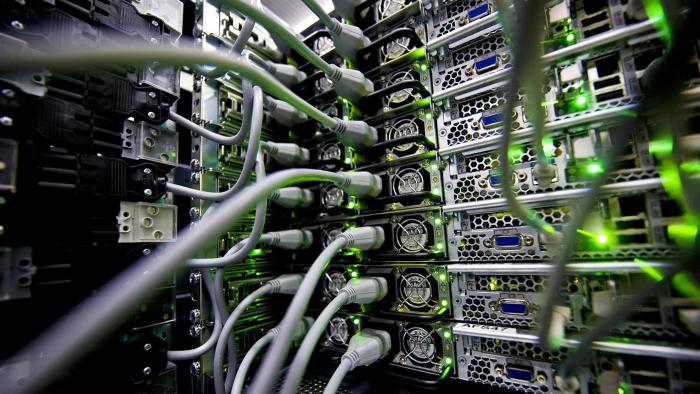
\includegraphics[width=0.9\textwidth]{Server_back.jpg}
            \end{column}
        \end{columns}
    \end{minipage}
\end{frame}

%------------------------------------------------

\begin{frame}
    \frametitle{Going Agile}
    \begin{minipage}[t]{0.95\textwidth}
        \begin{columns}
            \begin{column}{0.8\textwidth}
                Requirements started to grow
                \begin{itemize}
                    \item Agile approach was needed
                \end{itemize}
                Since a few years we started using Openstack to deploy virtual machines for our users and Puppet to configure the services 
            \end{column}
            \begin{column}{0.2\textwidth}
                
\includegraphics[width=0.9\textwidth]{openstack-logo512.png}
            \end{column}
        \end{columns}
    \end{minipage}
    \vspace{\belowdisplayskip}
    \vspace{\belowdisplayskip}
    \begin{minipage}[t]{0.95\textwidth}
        \begin{center}
        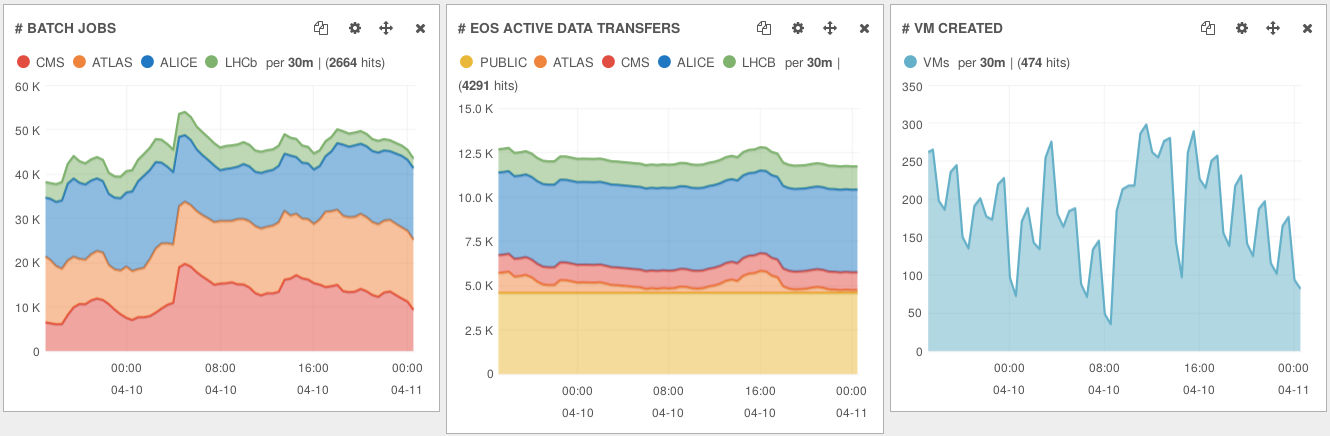
\includegraphics[width=0.83\textwidth]{Eos-CreatedVm.png}
    \end{center}
    \end{minipage}
\end{frame}

%------------------------------------------------
\section{Puppet @ CERN}
%------------------------------------------------

\subsection{Current Infrastructure}
\begin{frame}
    \frametitle{Current Setup}
    We started using Puppet a few years ago and, since then, things evolved a lot...

    We changed several time the configuration of our puppet masters in order to keep up with the requests and we found out that:

    \begin{itemize}
        \item Puppet scales horizontally quite well
        \item The NFS filer underneath … does not
    \end{itemize}
\end{frame}

%------------------------------------------------

\begin{frame}
    \frametitle{Clusters and Pools}
\end{frame}

%------------------------------------------------
\section{Configuration Management}
%------------------------------------------------

\subsection{Managing configuration changes}
\begin{frame}
    \frametitle{Git repositories}
\end{frame}

%------------------------------------------------

\begin{frame}
    \frametitle{QA workflow}
\end{frame}

%------------------------------------------------

\subsection{Tools}
\begin{frame}
    \frametitle{Continuous Integration}
\end{frame}

%------------------------------------------------

\begin{frame}
    \frametitle{Jens}
\end{frame}

%------------------------------------------------

\begin{frame}
    \frametitle{Mco}
\end{frame}

%------------------------------------------------

\begin{frame}
    \frametitle{Package Inventory}
\end{frame}

%----------------------------------------------------------------------------------------

\end{document} 
